\section{Värmeflöde genom grunden}

För att räkna på energin som flödar genom grunden är det nödvämdigt att räkna
transient. Detta då berget tar åt sig värme väldigt långsamt. I praktien innebär detta att ett statiskt jämviktsläge aldrig uppnås.

Problemet är behandlat med finita elementmetoden av värmeledningsekvationen.
Geometrin av problemet och trianguleringen kan ses i figur \ref{fig:foundation:tri}.
Randvärdena som är satt är att alla rander som går från berg till berg är adiabatiska.
Detta kommer inte stämma i praktiken om inte definitionsmängden sätts till oändligt
stor. För lösning av detta problem kan det dock ses som en tillräckligt god
approximation eftersom definitionsmängden är stor och temperaturen inte varierar så mycket
från förväntat värde.

Vid randerna mot grunden ligger ett neumannvillkor som säger att energiflödet är produkten
av temperaturdifferansen mellan temperaturen på randen och inomhustemperaturen på $\unit[20]{^\circ C}$.
Grundens U-värde har här satts till $U = 0,7/0,45 \approx \unit[1,556]{ Wm^{-2}K^{-1}}$. Detta värde är
baserat på att det ligger $\unit[0,25]{m}$ betong mellan källaren och grunden och att det ligger ytterligare $\unit[0,2]{m}$
betong mellan uppvärmda utrymmen och källaren. Vidare antas att det föreligger god omrörning i de båda
luftskikten vilket gör att de har $R=0$. Detta antagande är dock inte helt giltigt vilket leder till att kyleffekten
uppskattas vara något för hög.
Vid randerna till luft är konvektionsparametern satt
till $h = \unit[15,5]{Wm^{-2}K^{-1}}$. Detta är en siffra som motsvarar
en vindhastighet på ungefär $v = \unit[2]{ms^{-1}}$. Utomhustemperaturen har valts
som en minstakvadratanpassad trigonetrisk funktion av
medeltemperaturen de senaste tjugo åren vilket kan ses i figur
\ref{fig:foundation:meantemperature}. Anpassningen gör att
differentialekvationerna av galerkinformuleringen kan lösas analytiskt
för alla tider istället för att systemet ska behöva lösas semidiskret.
Detta minskade exekveringstiden dramatiskt vilket gav möjlighet att använda en
mycket finare triangulering. Dessutom kan alla termer i lösningen
som går mot noll då tiden går mot oändligeheten sättas till noll. Detta innebär
att få lösningar når ett transient jämviktsläge som liknar det jämviktsläge vi har i praktiken.
Initialvärdena kommer således inte ha någon betydelse och dessa kan då väljas
godtyckligt. 
För att uppnå detta resultat med semidiskret MOL behövs väldigt många itereringar för att
nå konvergens. Den resulterande koden kan ses i bilaga \ref{app:femfoundation}.

\begin{figure}
\centering
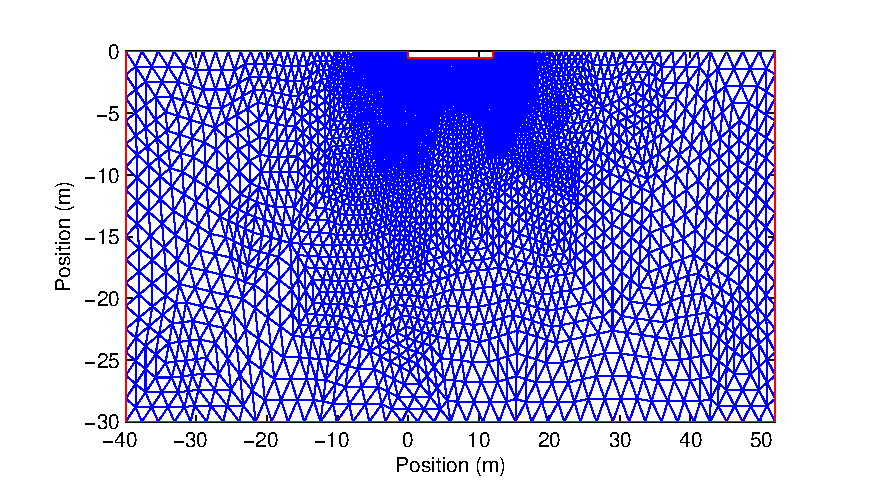
\includegraphics{images/trifoundation.eps}
\caption{Definitionsmängd och triangulering berget under grunden.}
\label{fig:foundation:tri}
\end{figure}


\begin{figure}
\centering
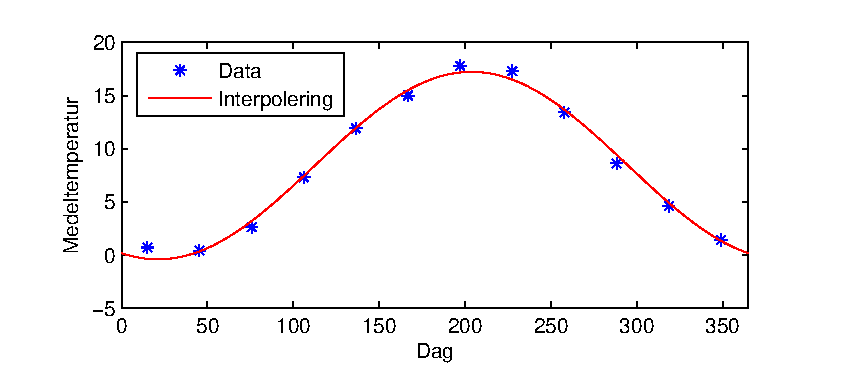
\includegraphics{images/meantemperature.eps}
\caption{
Medeltemperaturen för Göteborg de senaste 20 åren. Punkterna är data tagna från Miljöförvaltningen och linjen är minstakvadratanpassningen som senare använts för att beräkna energiflöden.}
\label{fig:foundation:meantemperature}
\end{figure}

%Miljöförvaltningen
%http://www4.goteborg.se/prod%5Csk%5Cstatistik%5CstatistikR5.nsf/0/3F002A395ED39AC8C1256D3B00393D0E/$File/3.01.pdf
